\chapter{Experimental Setup}
\minitoc
\section{The Large Hadron Collider at CERN}
An overview of the experimental setup used to collect data for this analysis is explained in the chapter. 
In this search, the proton-proton collision data recorded by the Compact Muon Solenoid (CMS) experiment at the Large Hadron Collider (LHC) at a center-of-mass energy of 13 TeV is used.
The chapter begins with a brief explanation of the LHC including the pre-accelerator complex. The different components and subsystems of the CMS detector will be discussed in Sec. \ref{sec:cms_ex}. The chapter will end with a description of the event simulation tools in Sec. \ref{sec:simulation}. 
%\newpage
\subsection{The CERN accelerator complex}
A particle accelerator is a machine that moves charged particles by using electromagnetic fields.  Nowadays, accelerator machines are using changing electromagnetic fields to propel particles to nearly the speed of light. 
The large hadron collider (LHC) is the world's largest particle accelerator and it is the last ring of the accelerator chain at CERN.  CERN is an abbriviation for the European Organization for Nuclear Research - Conseil Europ{\'e}en pour la Recherche Nucl{\'e}aire. 
The complex is situated about 100 meters below the ground, between the Jura Mountains and Lake Geneva. \\ 
Fig.\ref{fig:CERN_complex} shows the entire CERN accelerating complex including the storage rings, beam transfer
lines and four major LHC experiments. 
In this thesis, the data collected from the proton-proton collisions in LHC is used. The LHC is the final stage of a successive acceleration procedure of protons. The protons begin their journey in a hydrogen bottle which is currently at the beginning of the linear accelerator (LINAC2) which propels the particles to 50 MeV. This linear accelerator has served to many experiments at CERN since 1978 and it will be replaced by newly commissioned LINAC4  in 2020\cite{LINAC2}. The beams provided by the LINAC are then injected to the Proton Synchrotron Booster where the particles are further accelerated to 1.4 GeV \cite{Booster}. Next, the protons delivered by the Booster are accelerated up to 25 GeV by the Proton Synchrotron (PS) \cite{PS}. This accelerator is operating since 1959 and it is the first accelerator of CERN.
The last machine before the LHC is the Super Proton Synchrotron (SPS) \cite{SPS}, where the protons reach the energy of 450 GeV. The SPS was operating as a proton-antiproton collider from 1981 to 1984, which leads to the discovery of W \cite{Wboson} and Z \cite{Zboson} bosons. This journey of protons to reach the LHC takes 16 minutes in the current injection scheme \cite{LHCDR}.
%%%%%%
\begin{figure}
\begin{center}
\includegraphics[width=\textwidth]{Plots/LHC/cernComp.png}
\caption{\label{fig:CERN_complex} CERN accelerator complex \cite{CERN_complex}: }
\end{center}
\end{figure}
%%%%%%%%%5
\subsection{The Large Hadron Collider}
The LHC is primarily designed to collide protons at a center-of-mass energy of 14 TeV. The LHC tunnel is originally build for the LEP with a total circumference of 27 km.
After shutdown of the LEP the construction of LHC began in 2000 and the first beams were circulated in September, 2008. Due to an electrical malfucntion in the magnet system the first collisions are delayed until November, 2009. \\
The LHC incorporates different methods already probed at different synchrotrons worldwide at the same time pushing the limits even further. 
In total more than 9000 magnets are used in the LHC. 1232 of them are the main superconducting dipoles responsible for the bending of the beam. To focus the beam, superconducting quadrupole magnets are  used, while the remaining sextupole and higher order magnets are used to correct the beam chromaticity. \\
The proton bunches from SPS are injected to the two counter-rotating rings of the LHC with a 450 GeV. The beam acceleration take place at a point between ALICE and CMS experiments, where 16 superconducting cavities are mounted. Each beam gains an acceleration of 485 keV per turn, which provides the necessary acceleration to reach the 6.5 TeV in about 20 minutes at the moment. \\
The two beams collide in four intersection points where the detectors of the experiments are located.\\
For the interested reader, the LHC design details are introduced here \cite{LHCDR}. \\
\textbf{LHC parameters}\\
One important parameter of LHC relevant to the physics analyses is the particle density delivered by LHC which can be quantified with its {\it luminosity}. The instantanaous luminosity, which is denoted by $\mathcal{L}$, is estimated using a variaty of beam parameters:
\begin{equation}
  \label{eqn:Lum_inst}
  \mathcal{L} = \frac{N^2_pN_bf_{rev}\gamma_r}{4\pi\epsilon_n\beta^*}\rm F,
\end{equation}
where $N_p$ is the number of particles per bunch, $N_b$ is the number of bunches per beam, $f_{rev}$ is revolution frequency, $\gamma_r$ is relativistic gamma factor, $\epsilon_n$ is the normalized transverse beam emittance, and $\beta^*$ is the beta function at the interaction point. The parameter F is the reduction factor because of the beam crossing angle.\\
The total integrated luminocity over time can be calculated:
\begin{equation}
  \label{eqn:Lum}
  L = \int \mathcal{L} dt.
\end{equation}
Using the instantenous luminosity the expected event rate of a process can be computed:
\begin{equation}
  \label{eqn:Eventrate}
  \frac{dN}{dt} = \sigma \cdot \mathcal{L},
\end{equation}
where $\sigma$ is the cross section of a specific process.\\
At the design energy of 14 TeV and with a total bunch crossing rate of 40 MHz, a peak luminosy of $\mathcal{L}=10^{34}cm^{-2}s^{-1}$ would be achieved. However, to reach these conditions, prior studies and commissioning of the machine at lower levels should be performed. Therefore, the first proton-proton (pp) run of the LHC was performed at a centre-of-mass energy of 7 TeV with a peak luminosity of $\mathcal{L}=3.6 x 10^{33}cm^{-2}s^{-1}$. Total integrated luminosity of around 5 fb$^{-1}$ was delivered to the major ATLAS (A Toroidal LHC AparatuS) and CMS experiments until the end of 2011 \cite{lumi5}.
Next, following the 8 TeV run ({\it Run 1}) in 2012 the first long shutdown which took place for 1.5 year, allowed to accelerate protons to their current energy of 6.5 TeV. In 2015 the second LHC run, namely {\it Run 2}, has begun with a peak luminosity of $\mathcal{L}=5 x 10^{33}cm^{-2}s^{-1}$ at a bunch spacing of 25 ns.
A full list of the LHC parameters for the 13 TeV runs can be accessed here \cite{LHC_param}. The present analysis uses the data collected in 2016 with an integrated luminosity of 35.9 fb$^{-1}$ by CMS experiment.
\\
\textbf{The Future of the LHC}\\
According to the LHC plans, the current research programme will continue until 2023 including {\it Run 3} with 14 TeV center-of-energy and the target integrated luminosity is 500 fb$^{-1}$ \cite{LHC_time}.
LHC further future plans are constraint by the fixed ring size, thus the limited proton energy.  Therefore the LHC proceeds in the direction of the intensity frontline. High-Luminosity (HL-LHC) project is planned to start at the beginning of 2024. HL-LHC could reach luminosities of the order of $\mathcal{L}=10^{35}cm^{-2}s^{-1}$ which is hundred times more than the LHC design. The main challenge in this environment would be the development of new magnet system to handle with such an increase in number of protons per beam.
\newpage
\section{The Compact Muon Solenoid experiment at the LHC}
\label{sec:cms_ex}
The Compact Muon Solenoid (CMS) \cite{CMS_TDR} detector is a multi-purpose device to operate at the LHC. CMS is installed about 100 metres underground close to the French village of Cessy.
The first Letter of Intent for the CMS detector was published in 1992 \cite{CMS_FirstLet}, it was followed by the construction of the individual components soon afterwards. \\
As it can be seen from the Fig. \ref{fig:CMS}, CMS detector is in onion shape, meaning it incorporates successive layers. These layers which are corresponding to various purpose sub-detectors can be listed as follows: the inner tracking system is surrounding the interaction point; afterwards the electromagnetic and hadron calorimeters are located between the tracker and 6m wide solenoid magnet. Outermost layer is the extensive system of muon trackers which infact makes up more than 80\% of the detector volume. In addition to these, forward calorimeters are placed along the beam-pipe immediately after the muon detectors.\\
\textbf{Coordinate system and the relevant kinematic variables}\\
The origin is centered at the nominal collision point inside the experiment. The y-axis pointing vertically upward, and the x-axis pointing radially inward toward the center of the LHC. Therefore, the z-axis points along the beam direction following the direction of the counter-clockwise rotating beam. Due to the almost symmetric cylindrical shape of the detector, generally, cylindrical coordinate system is used. 
In other words, the same z-axis with the 2-D polar coordinates, which involve the radial distance r and azimuthal angle $\phi$, is used. The polar angle $\theta$ is measured from the z-axis.\\
The pseudorapidity $\eta$, derived from the $\theta$, is also a widely used variable and it characterizes the boost of the particles:
\begin{equation}
  \label{eqn:Eta}
   \eta = {\rm -ln [tan(\frac{\theta}{2})]}.
\end{equation}
The pseudorapidity is a version of rapidity, which is Lorentz invariant under longitudinal – along the beam axis - boosts. In the case where particle masses are negligible, rapidity converges to $\eta$.\\
Another variable used commonly is the spacial distance:
\begin{equation}
  \label{eqn:DR}
   \Delta R = \sqrt{(\Delta\eta)^2+(\Delta\phi)^2}.
\end{equation}
The proton is a composite particle, which includes partons. Therefore, the proton-proton collisions are interactions of the corresponding partons. Furthermore, even though the energy of the incoming proton beams are symmetric, this condition does not necessarily need to be hold for individual partons. Therefore, the total center-of-mass energy is an unpredictable quantity of an event. However, since the incoming protons, therefore the partons, are aligned along the beam axis, the total momentum in the transverse
plane is close to be zero, which is followed also by the momentum conservation of the collision remnants. As a result of this, the transverse momentum of the particles, $\sqrt{p^2_x+p^2_y}$, are extremely useful for the physics analyses.
\begin{figure}
\begin{center}
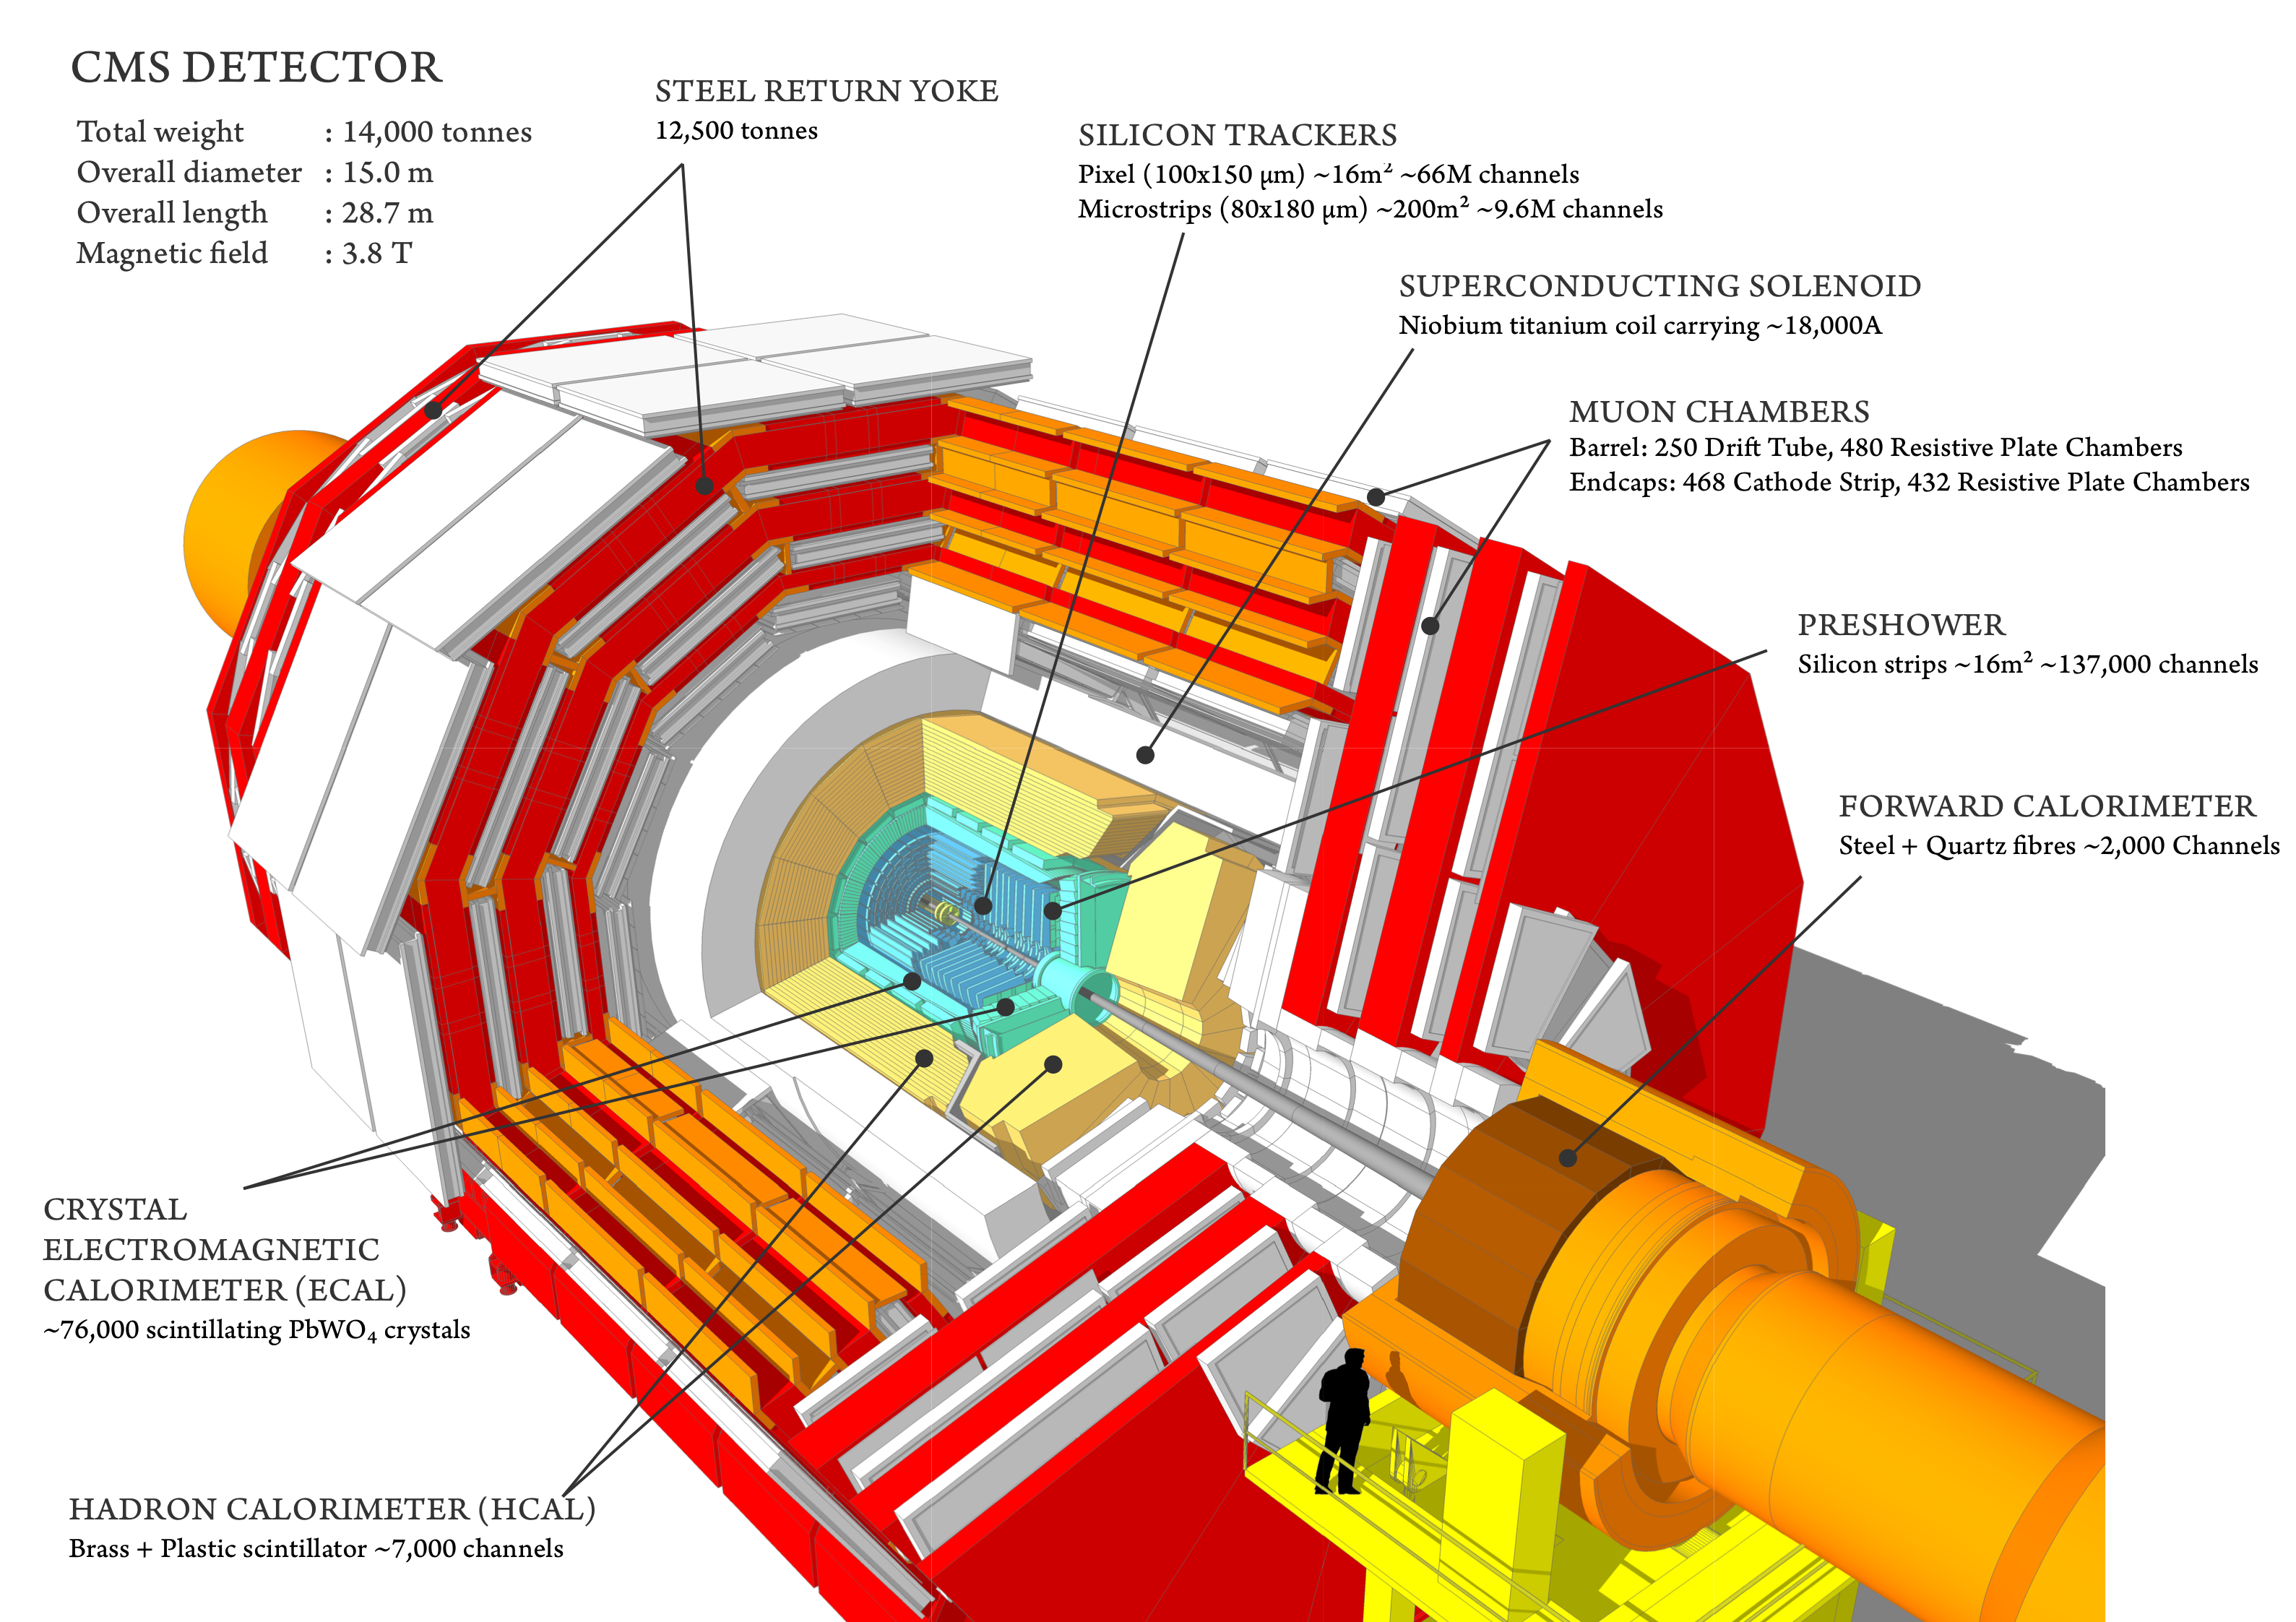
\includegraphics[width=0.9\textwidth]{Plots/CMS/CMS.jpg}
%\vspace{-5cm}
\caption{\label{fig:CMS} Schematic view of the CMS detector with a cut-out quadrant \cite{CMS_Vis}}
\end{center}
\end{figure}
\subsection{Superconducting Magnet}
As it can be understood from the name of the CMS experiment, the solenoid magnet is a crucial component of the detector. It has an important role in precise measurements of charged particles. It is designed to host the tracker and calorimeter systems at the same time providing a uniform axial magnetic field of 4T within its volume. Due to its unique design and not yet well-understood aging, it is currently being operated at slightly lower field strength of 3.8T. Further information on the measurement of the magnetic field inside the  barrel yoke can be found here \cite{CMS_Mag}.
\subsection{Tracker}
The inner tracking system comprises the innermost part of the CMS experiment. The main purpose of this component is the identification and measurement of tracks ascending from charged particles coming from the interaction vertices. This detector system has several restraint requirements in terms of detection efficiency, spacial resolution and radiation safety due to the large collision rates and high particle multiplicities.\\
To overcome these challanges, the tracker system consists of silicon pixel and strip sensors.\\
The Silicon Pixel detector is located just around the interaction region. It covers a pseudorapidity range of $|\eta|$$<$2.5.
%\newpage
\subsection{Electromagnetic Calorimeter}
The succeeding sub-detector to the inner tracker is the electromagnetic calorimeter (ECAL). ECAL is a hermetic homogeneous detector, which is composed of lead tungstate (PbWO$_4$) crystals. The lead tungstate scintillators leads to a compact calorimeter design, which is important to cope with the space restrictions inside the magnet. The ECAL consists of endcap components on each side and a barrel part. The barrel coveres a range of $|\eta|<$1.479 and the endcap extends the range until $|\eta|$$=$3.0. Additionally, a preshower detector is installed in front of the endcap. The main purpose of the ECAL is to measure the energy of electrons and photons coming from the tracking system. The preshower prevents the misidentification of photons in ECAL originating from neutral pion decays. To detect the showers produced in the crystals in the barrel and endcap, photodiodes and phototriodes are used respectively.
The energy resolution of ECAL barrel is measured to be \cite{ECAL_res}:
% \renewcommand{\arraystretch}{1.5}
\begin{equation}
  \label{eqn:EcalRes}
   (\frac{\sigma}{E})^2 = (\frac{2.8\%}{\sqrt{E}})^2+(\frac{0.12}{E})^2+(0.30\%)^2 ,
\end{equation}
 %\renewcommand{\arraystretch}{1.0}
where the three contributions correspond to the stochastic, noise, and constant terms. The constant terms cover the non-uniformities, intercalibration errors and energy leakage from the back of the crystal. According to this formula, a 100 GeV electron can be measured with a resolution of 0.4\%.
%\newpage
\subsection{Hadronic Calorimeter}
The Hadron Calorimeter (HCAL) is installed directly after ECAL without any dead material in between.
The principle purpose of the HCAL is to measure the energy of hadrons, which are particles consist of quarks and gluons.
The HCAL is a sampling calorimeter in other words it finds a particle’s position, energy and arrival time using layers of brass and scintillator plates. When the particle passes through from these layers, a rapid light pulse is produced. Then optic fibers feed the light into readout boxes where photodetectors amplify the signal. A particle’s energy is then measured by summing over the amount of light in a given region of many layers of strips in depth, which is called HCAL tower.
HCAL has two components inside the solenoid: the barrel (HB) part covers a pseudorapidity range of $|\eta|<$1.3 and the endcap (HE) is placed in the range of 1.3$<|\eta|<$3. There is an outer hadron calorimeter (HO) just after the magnet to stop the particles surviving after the HB; therefore this component is also known as a tail catcher. HO utilizes the material of the magnet as an absorber. In addition to the central part, the coverage of HCAL is extended by a very forward calorimeter (HCAL). The HF is installed outside the CMS endcaps at a distance of $|z|=\pm$11.2m from the collision vertex. The pseudorapidity range of HF is 2.85$<|\eta|<$ 5.19, thus it is expected that the HF is exposed to extreme particle flux. Aforementioned leads to a choice of radiation-hard technology: steel is used as absorber material while quartz-fibers are used as active material.
\subsection{Muon System}
The importance of the muon system has been stressed out in the name of the CMS experiment.
Muon system has three major roles: identification, measurement of momentum and triggering of muons. A combination of three different particle detectors is utilized to achieve these goals. In barrel region the magnetic field is uniform and the muon flux is low. Therefore, drift tubes are used in this section corresponding to a pseudorapidity range of $|\eta|<$1.2. The drift tube system serves as tracking detectors by measuring the electromagnetic cascades accompaning the muons. Outside of the barrel yoke, towards the endcaps, the magnetic field becomes stronger and non-uniform. Moreover, particle flux increases in this region. Therefore, the detectors in the endcaps have to be fast and radiation hard. To overcome these challenges finely segmented cathode strip chambers (CSC), which are located in the pseudorapidity range 0.9 $<|\eta|<$2.4, are used. CSCs are used to measure the radial position of muons. In addition to drift tubes and cathode strip chambers, the resistive plate chambers are installed to supplement the triggering system in a fast and independent way.
In the muon reconstruction, informations from the tracker and muon systems are used together to attain the best momentum resolution. 
\subsection{Trigger and Data Acquisition Systems }
Given the 25ns time interval between the proton bunches, the collision rate inside the detector reaches up to 45MHz.  An event with all the measured information occupies about 1 MB in size. To save all events, a bandwidth of 60TB/s would be needed. However, achieving such high transmission of data is impossible with today’s technology. Therefore, a trigger system is necessary to select the most interesting events. The CMS trigger system is composed of two levels. The first level (L1) utilizes the information from the calorimeters and muon detectors. It consists of custom hardware processors. The accepted events are then sent with an output rate of maximum 100kHz to the second level, which is also known as High Level Trigger (HLT). The main purpose of HLT is to reconstruct physics object and to define events with inter- esting features. In the HLT stage, events are discarded as soon as the available information is enough to take the decision before being fully reconstructed. The HLT further decreases the event rate to an order of magnitute 100 Hz before storage. The HLT requires an immense parallelism to handle the event rate coming from L1 trigger.
\subsection{Luminosity measurement}
\label{sec:luminosity}
%Luminosity measurement and the unceartinity on it are important measurement that will be touched shortly again in the systematics chapter
Luminosity information is essential for both the beam parameters and physics analysis. For physics analysis, the integrated luminosity is related to the number of events of a certain process through Eqn. \ref{eqn:Eventrate}. The instantaneous luminosity is measured using two dedicated detectors: the Fast Beam Condtions Monitore (BCM1f) \cite{LUMTECH} and the Pixel Luminosity Telescope (PLT).  In addition to dedicated detectors, the pixel tracker, drift tubes and hadron forward calorimeter systems are used as well. \\
In this thesis, the total data collected by the CMS experiment corresponds to a 35.9 fb$^{-1}$ integrated luminosity and uncertainty on it is measured to be 2.6\% \cite{lumi1}.
%\subsection{Future of CMS}
%upgrade plans.. pixel .. will help to motivate future of physics analysis
%\newpage
\section{Event simulation}
\label{sec:simulation}
Monte Carlo (MC) simulations provide events close-to-reality. Both the experimental and theoretical physics searches benefit from MC simulations to study the dedicated physics processes as well as the detector methods.
In the following, a short overview of simulation technics used in this analysis is presented.
\subsection{Event generation}
The simulation of proton-proton collisions is an extrimely difficult task due to the composite structure of protons. This complicated task can be divided into stages with decreasing energy scale.\\
First, the scattering amplitude is computed using the matrix element (ME) where the proton parton distribution functions (PDFs) are used to describe the initial state momenta of partons. Naturally, being the first step, the hardest particles of the collision are produced in this stage.
Second, the initial-state radiation (ISR) and final-state radiation (FSR) are modeled in the parton shower stage. In parton shower, relative transverse momenta evolve from a high scale to lower values. Here an infrared cutoff on the parton showers is needed due to the perturbation theory. Finally, hadrons are formed using hadronization models.\\
MC samples used in this thesis are simulated with the $\MADGRAPH$5\_\textsc{aMC@}NLOv2.2.2 or v.2.3.3 \cite{MADGRAPH} and POWHEGv2.0 \cite{POWHEG1,POWHEG2,POWHEG3,POWHEG4,POWHEG5}. Further details are given in Sec. \ref{sec:bkg_proc} when separate background processes are discussed.
A more profound introduction to MC generators used in LHC physics can be found in \cite{EventGen1}.
\subsection{Detector simulation}
The final state particles, which are emerging after the generation, showering and hadronization states are required to be propagated to detector simulation.  This stage involves the modeling of interactions between those particles and the detector hardware material as well as the readout electronics of CMS. 
In CMS the main technic is called Full simulation, for which the GEometry ANd Tracking (GEANT4) toolkit is used \cite{GEANT}.
However, the Full simulation requires massive computer power; as a result, for large-scale MC production, like SUSY parameter phase scans, a more effective technic is necessary. 
Therefore, CMS established a Fast Simulation (FastSim) software \cite{fastsim}. Several features of the detector geometry and particle-matter interactions are simplified to increase the computational power. Detector responses of FastSim samples are tuned to match to the full simulation. 
%\lipsum